\documentclass[11pt,a4paper]{article}
\usepackage[utf8]{inputenc}
\usepackage[T1]{fontenc}
\usepackage{lmodern}
\usepackage[spanish,es-noshorthands]{babel}
\usepackage{microtype}
\usepackage[a4paper,margin=2.3cm]{geometry}
\usepackage{booktabs,array,longtable}
\usepackage{graphicx,caption}
\usepackage{float}
\usepackage{amsmath}
\usepackage{xcolor}
\usepackage{listings}
\usepackage{enumitem}
\usepackage{fancyhdr}
\usepackage{xurl}
\usepackage{hyperref}
\usepackage{tikz}
\usetikzlibrary{arrows.meta,positioning,shapes.geometric,fit,calc}

\hypersetup{colorlinks=true,linkcolor=blue!50!black,urlcolor=blue!60!black,
  pdftitle={Anexo del Entregable 1 -- Guía de uso del pipeline smn\_toe},
  pdfauthor={Jonathan Aaron Paredes Quispe}}
\hyphenpenalty=10000
\exhyphenpenalty=10000
\setlength{\emergencystretch}{3em}
\urlstyle{tt}
\newcommand{\archivo}[1]{\begingroup\hypersetup{urlcolor=black}\url{#1}\endgroup}
\newcolumntype{L}[1]{>{\raggedright\arraybackslash}p{#1}}
% Macros compartidas entre el informe revisado y las auditorias.
% Cifras verificadas contra los archivos del repositorio (ver A01/A04/A07):
\newcommand{\nUniverso}{102}   % source_id CMIP6 con tos/Omon en ESGF (00b, model_availability_priority.csv)
\newcommand{\nSeed}{41}        % publican los cuatro experimentos (config/models_seed_cmip6.csv)
\newcommand{\nSel}{40}         % completos + QC PASS (models_inventory_final.csv)
\newcommand{\nComb}{160}       % combinaciones modelo-experimento PASS (qc_report.csv)
\newcommand{\nNoEnc}{44}       % config/models_no_encontrado_44.csv
\newcommand{\nParcial}{18}     % 102 - 40 - 44
% Fecha de la portada: fija (no \today), editable en un solo lugar.
\newcommand{\fechaentrega}{28 de septiembre de 2026}
% Estado de codigo que documenta el E1 (antes de los cambios del E2)
\newcommand{\commitEone}{\texttt{8ee6184}}

\graphicspath{{../}}
\setlength{\parskip}{0.45em}
\setlength{\parindent}{0pt}
\pagestyle{fancy}
\fancyhf{}
\fancyhead[L]{\small Anexo del Entregable N.\textsuperscript{o}~1 -- Guía de uso del \emph{pipeline}}
\fancyhead[R]{\small \thepage}
\renewcommand{\headrulewidth}{0.4pt}
\setlength{\headheight}{14pt}

% Colores (tinta neutra + un azul de acento)
\definecolor{acento}{HTML}{2A78D6}
\definecolor{tinta}{HTML}{0B0B0B}
\definecolor{tinta2}{HTML}{52514E}
\definecolor{fondocaja}{HTML}{F3F6FB}
\definecolor{terminal}{HTML}{1E1E1E}
\definecolor{verde}{HTML}{1BAF7A}
\definecolor{ambar}{HTML}{EDA100}

% Bloques de comandos: fondo claro, se pueden copiar
\lstdefinestyle{comando}{basicstyle=\ttfamily\small,backgroundcolor=\color{fondocaja},
  frame=single,rulecolor=\color{acento!40},framesep=6pt,xleftmargin=6pt,xrightmargin=6pt,
  breaklines=true,columns=fullflexible,keepspaces=true,showstringspaces=false,
  literate={á}{{\'a}}1 {é}{{\'e}}1 {í}{{\'i}}1 {ó}{{\'o}}1 {ú}{{\'u}}1 {ñ}{{\~n}}1}
\lstset{style=comando}

% Caja de aviso
\newcommand{\aviso}[2]{\par\noindent\begin{tikzpicture}
\node[draw=#1!70,fill=#1!8,rounded corners=3pt,inner sep=7pt,text width=\dimexpr\linewidth-16pt\relax,align=left]{#2};
\end{tikzpicture}\par}

\begin{document}

\begin{titlepage}
\centering
\noindent\rule{\textwidth}{0.6pt}
\vspace{1.4cm}

{\Large\bfseries ANEXO DEL ENTREGABLE N.\textsuperscript{o}~1\par}
\vspace{0.6cm}
{\large Guía de uso del \emph{pipeline} de datos \texttt{smn\_toe}\par}
\vspace{1.2cm}
\rule{0.7\textwidth}{0.6pt}
\vspace{1.2cm}

{\normalsize\bfseries Concepto:\par}
\vspace{0.3cm}
{\normalsize Servicio de asistencia en temas de investigación para evaluar\\
la influencia del cambio climático en los eventos de El Niño\\
y sus impactos en el Perú\par}
\vspace{1.2cm}
{\small Prestado para: Servicio Nacional de Meteorología e Hidrología del Perú -- SENAMHI\par}
\vspace{1.2cm}
\begin{minipage}{0.8\textwidth}\small\centering
Este anexo acompaña al informe del Entregable~1. Explica cómo instalar y ejecutar el \emph{pipeline}, qué produce, cuánto tarda y cómo se usarán sus resultados en los entregables siguientes. Está escrito para quien usa Linux de forma básica: cada comando se puede copiar tal cual. El repositorio es de libre acceso.
\end{minipage}
\vfill
{\small\bfseries Responsable:\par}
{\small Ing. Jonathan Aaron Paredes Quispe\par}
\vspace{0.4cm}
{\small\bfseries FECHA: \fechaentrega\par}
\vspace{0.6cm}
\noindent\rule{\textwidth}{0.6pt}
\end{titlepage}

\tableofcontents
\clearpage

% ============================================================
\section{Qué hace el \emph{pipeline}}
% ============================================================

El \emph{pipeline} reúne en un único formato comparable la temperatura superficial del mar (TSM) de los modelos climáticos CMIP6 y la observación ERSSTv5. Descarga los datos de internet, los lleva a una misma grilla, calendario, unidad (°C) y máscara de océano, y verifica que estén completos. Todo se hace con un solo comando, \texttt{./run.sh}. La Figura~\ref{fig:que} resume el recorrido.

\begin{figure}[H]
\centering
\begin{tikzpicture}[
  font=\small,
  fuente/.style={draw=tinta2,fill=white,rounded corners=3pt,text width=2.7cm,align=center,minimum height=1.0cm},
  etapa/.style={draw=acento,fill=acento!10,rounded corners=3pt,text width=3.1cm,align=center,minimum height=1.25cm},
  producto/.style={draw=verde!80!black,fill=verde!10,rounded corners=3pt,text width=3.2cm,align=center,minimum height=1.0cm},
  flecha/.style={-{Latex[length=2.5mm]},thick,tinta2}]
\node[fuente] (esgf) at (0,1.5) {ESGF\\\scriptsize modelos CMIP6};
\node[fuente] (cds) at (0,0) {Copernicus CDS\\\scriptsize respaldo};
\node[fuente] (noaa) at (0,-1.5) {NOAA PSL\\\scriptsize ERSSTv5 observado};
\node[etapa] (e1) at (4.1,1.9) {\textbf{1. Buscar}\\\scriptsize pasos 00, 00b, 01\\ qué modelos existen};
\node[etapa] (e2) at (4.1,0.3) {\textbf{2. Descargar}\\\scriptsize pasos 02, 03};
\node[etapa] (e3) at (4.1,-1.3) {\textbf{3. Homogeneizar}\\\scriptsize pasos 04, 05\\ grilla, °C, máscara};
\node[etapa] (e4) at (4.1,-2.9) {\textbf{4. Verificar}\\\scriptsize pasos 06, 07\\ control de calidad};
\node[producto] (p1) at (8.7,1.1) {\textbf{40 modelos}\\\scriptsize $\times$ 4 experimentos listos\\ \texttt{data/processed/}};
\node[producto] (p2) at (8.7,-0.4) {\textbf{Inventario y QC}\\\scriptsize tablas CSV};
\node[producto] (p3) at (8.7,-1.9) {\textbf{Figuras y reporte}\\\scriptsize \texttt{figures/}, \texttt{logs/}};
\draw[flecha] (esgf.east) -- (e1.west);
\draw[flecha] (esgf.east) -- (e2.west);
\draw[flecha] (cds.east) -- (e2.west);
\draw[flecha] (noaa.east) -- (e2.west);
\draw[flecha] (e1) -- (e2);
\draw[flecha] (e2) -- (e3);
\draw[flecha] (e3) -- (e4);
\draw[flecha] (e4.east) -- (p1.west);
\draw[flecha] (e4.east) -- (p2.west);
\draw[flecha] (e4.east) -- (p3.west);
\node[draw=acento,dashed,rounded corners=4pt,inner sep=5pt,fit=(e1)(e4),label={[font=\scriptsize\ttfamily,text=acento]above:./run.sh}] {};
\end{tikzpicture}
\caption{Recorrido de los datos: tres fuentes en internet, cuatro etapas automáticas dentro de \texttt{run.sh} y tres tipos de producto.}
\label{fig:que}
\end{figure}

Los productos alimentan directamente el Entregable~2. Los números de paso (00 a 07) son los que usa el informe y los que acepta \texttt{run.sh} para ejecutar solo una parte (Sección~\ref{sec:ejecutar}).

% ============================================================
\section{Qué se necesita}
% ============================================================

\begin{center}\small
\begin{tabular}{@{}L{3.6cm}L{\dimexpr\textwidth-3.6cm-2\tabcolsep\relax}@{}}
\toprule
Requisito & Detalle \\
\midrule
Sistema operativo & Linux (probado en Ubuntu y en un clúster HPC). \\
Espacio en disco & Unos \textbf{90\,GB libres}: 73\,GB de datos crudos, cerca de 9\,GB de datos procesados e intermedios y margen. Se comprueba con \texttt{df -h .} \\
Conexión a internet & Estable. La descarga completa toma del orden de 13 horas. \\
Conda (Miniconda) & Gestor de programas; instala Python, CDO y el resto de las dependencias (Sección~\ref{sec:instalar}). \\
Repositorio & \archivo{https://github.com/Japq91/smn_toe}, de libre acceso. \\
Cuenta de Copernicus & \textbf{Opcional}. Solo se usa para los modelos que ESGF no resuelve; sin ella, ese paso se omite y el resto sigue. \\
\bottomrule
\end{tabular}
\end{center}

% ============================================================
\section{Instalación (una sola vez)}
\label{sec:instalar}
% ============================================================

Abra una terminal (en Ubuntu: \texttt{Ctrl+Alt+T}) y siga estos pasos en orden.

\textbf{Paso 1. Instalar Miniconda} (omitir si el comando \texttt{conda} ya existe; se comprueba con \verb|conda --version|):
\begin{lstlisting}
wget https://repo.anaconda.com/miniconda/Miniconda3-latest-Linux-x86_64.sh
bash Miniconda3-latest-Linux-x86_64.sh
\end{lstlisting}
Acepte la licencia y las opciones por defecto. Al terminar, \textbf{cierre la terminal y abra una nueva}.

\textbf{Paso 2. Descargar el repositorio} y entrar a su carpeta:
\begin{lstlisting}
git clone https://github.com/Japq91/smn_toe.git
cd smn_toe
\end{lstlisting}

\textbf{Paso 3. Crear el entorno de programas} (tarda unos minutos y se hace una sola vez):
\begin{lstlisting}
conda env create -f environment.yml
\end{lstlisting}
Esto crea el entorno \texttt{smn\_toe} con Python~3.11, CDO~2.1.1, \texttt{netCDF4}, \texttt{xarray}, \texttt{matplotlib}, \texttt{cartopy} y \texttt{cdsapi}. No hace falta activarlo a mano: \texttt{run.sh} lo activa solo.

\textbf{Paso 4 (opcional). Credenciales de Copernicus.} Cree una cuenta en \archivo{https://cds.climate.copernicus.eu}, acepte la licencia del conjunto \texttt{projections-cmip6} y guarde su clave personal en el archivo \texttt{\textasciitilde/.cdsapirc}:
\begin{lstlisting}
url: https://cds.climate.copernicus.eu/api
key: SU-CLAVE-PERSONAL
\end{lstlisting}

% ============================================================
\section{Ejecutar}
\label{sec:ejecutar}
% ============================================================

\subsection{La forma general}

\begin{lstlisting}
./run.sh [PASO_DESDE] [PASO_HASTA] [MAX_MODELOS]
\end{lstlisting}

Los tres valores son opcionales. Sin ninguno, se ejecuta todo: pasos \texttt{00 00b 01 02 03 04 05 06 07}, en ese orden. \texttt{PASO\_DESDE} y \texttt{PASO\_HASTA} limitan el rango de pasos. \texttt{MAX\_MODELOS} procesa solo los primeros $N$ modelos, lo que sirve para una prueba rápida.

\begin{center}\small
\begin{tabular}{@{}L{4.4cm}L{\dimexpr\textwidth-4.4cm-2\tabcolsep\relax}@{}}
\toprule
Comando & Para qué sirve \\
\midrule
\texttt{./run.sh 00 04 2} & \textbf{Prueba rápida}: todo hasta el regrillado, con solo 2 modelos. Úsela la primera vez para comprobar la instalación. \\
\texttt{./run.sh} & \textbf{Corrida completa}. La primera vez tarda del orden de 16 horas (Sección~\ref{sec:tiempos}). \\
\texttt{./run.sh 06 07} & Repetir solo el control de calidad y el inventario (minutos). \\
\texttt{./run.sh 07 07} & Regenerar inventario, figuras, reporte y paquete sin tocar los datos. \\
\bottomrule
\end{tabular}
\end{center}

\aviso{acento}{\textbf{Si la corrida se corta} (corte de luz, de red, o se cierra la terminal), basta con volver a ejecutar el mismo comando. Cada paso detecta lo que ya está hecho y continúa desde ahí, sin repetir descargas.}

\subsection{Elegir el comando}

\begin{figure}[H]
\centering
\begin{tikzpicture}[font=\small,
  preg/.style={draw=tinta2,fill=white,rounded corners=3pt,text width=3.9cm,align=center,minimum height=0.9cm},
  cmd/.style={draw=acento,fill=acento!10,rounded corners=3pt,text width=3.3cm,align=center,minimum height=0.9cm,font=\small\ttfamily},
  flecha/.style={-{Latex[length=2.3mm]},thick,tinta2},
  lbl/.style={font=\scriptsize,text=tinta2}]
\node[preg] (q1) at (0,0) {¿Es la primera vez en esta máquina?};
\node[cmd] (c1) at (5.2,0) {./run.sh 00 04 2};
\node[preg] (q2) at (0,-1.8) {¿Quiere todos los datos?};
\node[cmd] (c2) at (5.2,-1.8) {./run.sh};
\node[preg] (q3) at (0,-3.6) {¿Solo cambió el control de calidad?};
\node[cmd] (c3) at (5.2,-3.6) {./run.sh 06 07};
\node[preg] (q4) at (0,-5.4) {¿Solo quiere figuras y reportes al día?};
\node[cmd] (c4) at (5.2,-5.4) {./run.sh 07 07};
\draw[flecha] (q1) -- node[lbl,above]{sí} (c1);
\draw[flecha] (q1) -- node[lbl,right]{no} (q2);
\draw[flecha] (q2) -- node[lbl,above]{sí} (c2);
\draw[flecha] (q2) -- node[lbl,right]{no} (q3);
\draw[flecha] (q3) -- node[lbl,above]{sí} (c3);
\draw[flecha] (q3) -- node[lbl,right]{no} (q4);
\draw[flecha] (q4) -- node[lbl,above]{sí} (c4);
\draw[flecha,dashed] (c1.south) -- node[lbl,right]{si la prueba salió bien} (c2.north);
\end{tikzpicture}
\caption{Qué comando usar según la situación.}
\end{figure}

\subsection{Dejarlo corriendo en segundo plano}

Como la corrida completa dura muchas horas, conviene lanzarla de modo que siga aunque se cierre la terminal:
\begin{lstlisting}
nohup ./run.sh > logs/corrida.txt 2>&1 &
\end{lstlisting}
Para ver el avance en cualquier momento (se sale con \texttt{Ctrl+C}, sin detener la corrida):
\begin{lstlisting}
tail -f logs/pipeline.log
\end{lstlisting}

\subsection{Qué aparece en pantalla}

Antes de empezar, \texttt{run.sh} muestra un \textbf{reporte previo} con lo que ya existe (\texttt{[OK]}) y lo que falta (\texttt{[FALTA]}), junto con una estimación de tiempo basada en corridas anteriores en la misma máquina. La Figura~\ref{fig:terminal} muestra la salida real en la máquina de desarrollo, con los 40 modelos ya procesados.

\begin{figure}[H]
\centering
\begin{tikzpicture}
\node[fill=terminal,rounded corners=4pt,inner sep=9pt,text width=0.93\textwidth,align=left,font=\ttfamily\scriptsize,text=white] (t) {%
\textcolor{gray!60}{\$} ./run.sh\\[2pt]
=== Estado antes de esta corrida (run.sh) ===\\
\textcolor{verde}{[OK]}\ \ \ \ 00b\ \ \ config/models\_seed\_cmip6.csv (lista de modelos)\\
\textcolor{verde}{[OK]}\ \ \ \ 01\ \ \ \ data/interim/models\_catalog\_status.csv (catalogo ESGF)\\
\textcolor{verde}{[OK]}\ \ \ \ 02\ \ \ \ Descarga CMIP6: 160/160 combinaciones modelo x experimento\\
\textcolor{verde}{[OK]}\ \ \ \ 04/05 Grilla comun + mascara: 160/160 archivos\\
\textcolor{verde}{[OK]}\ \ \ \ 03\ \ \ \ data/raw/ersstv5/ersstv5\_region.nc (observado)\\
\textcolor{verde}{[OK]}\ \ \ \ 06\ \ \ \ data/processed/qc\_report.csv (control de calidad)\\
\textcolor{verde}{[OK]}\ \ \ \ 07\ \ \ \ data/processed/models\_inventory\_final.csv (inventario final)\\
==============================================\\[2pt]
\textcolor{gray!60}{\# en una máquina nueva, cada línea diría por ejemplo:}\\
\textcolor{ambar}{[FALTA]} 00b\ \ \ config/models\_seed\_cmip6.csv (lista de modelos) -{}- sin corridas previas en esta maquina, no se puede estimar
};
\end{tikzpicture}
\caption{Reporte previo de \texttt{run.sh} (salida real; la última línea ilustra el caso de una máquina nueva).}
\label{fig:terminal}
\end{figure}

Durante la corrida pueden aparecer dos preguntas, ambas con límite de 15 segundos. No hace falta responderlas: si nadie contesta, el \emph{pipeline} continúa solo.

\begin{center}\small
\begin{tabular}{@{}L{6.8cm}L{\dimexpr\textwidth-6.8cm-2\tabcolsep\relax}@{}}
\toprule
Pregunta & Si no se responde \\
\midrule
¿Buscar en nodos alternativos de ESGF y en Copernicus? [S/n] & Sí busca. Solo aparece si faltan modelos. \\
¿Regenerar las figuras que ya existen? & No regenera; conserva las figuras existentes. \\
\bottomrule
\end{tabular}
\end{center}

\aviso{ambar}{\textbf{Figuras desactualizadas.} Si cambia el conjunto de modelos, las figuras que ya existen \emph{no} se actualizan solas. Responda ``s'' a la segunda pregunta o borre la figura concreta en \texttt{figures/} antes de ejecutar \texttt{./run.sh 07 07}.}

% ============================================================
\section{Cuánto tarda}
\label{sec:tiempos}
% ============================================================

La Figura~\ref{fig:tiempos} muestra lo que tardó cada paso en la máquina de desarrollo cuando tuvo que hacer todo el trabajo. La descarga domina: una primera corrida completa toma en total del orden de \textbf{16 horas}. Las corridas siguientes tardan segundos o minutos, porque cada paso omite lo que ya está hecho. El Paso~03 (ERSSTv5) no aparece porque no hay una medición de su primera descarga; es un único archivo de unos 160\,MB.

\begin{figure}[H]
\centering
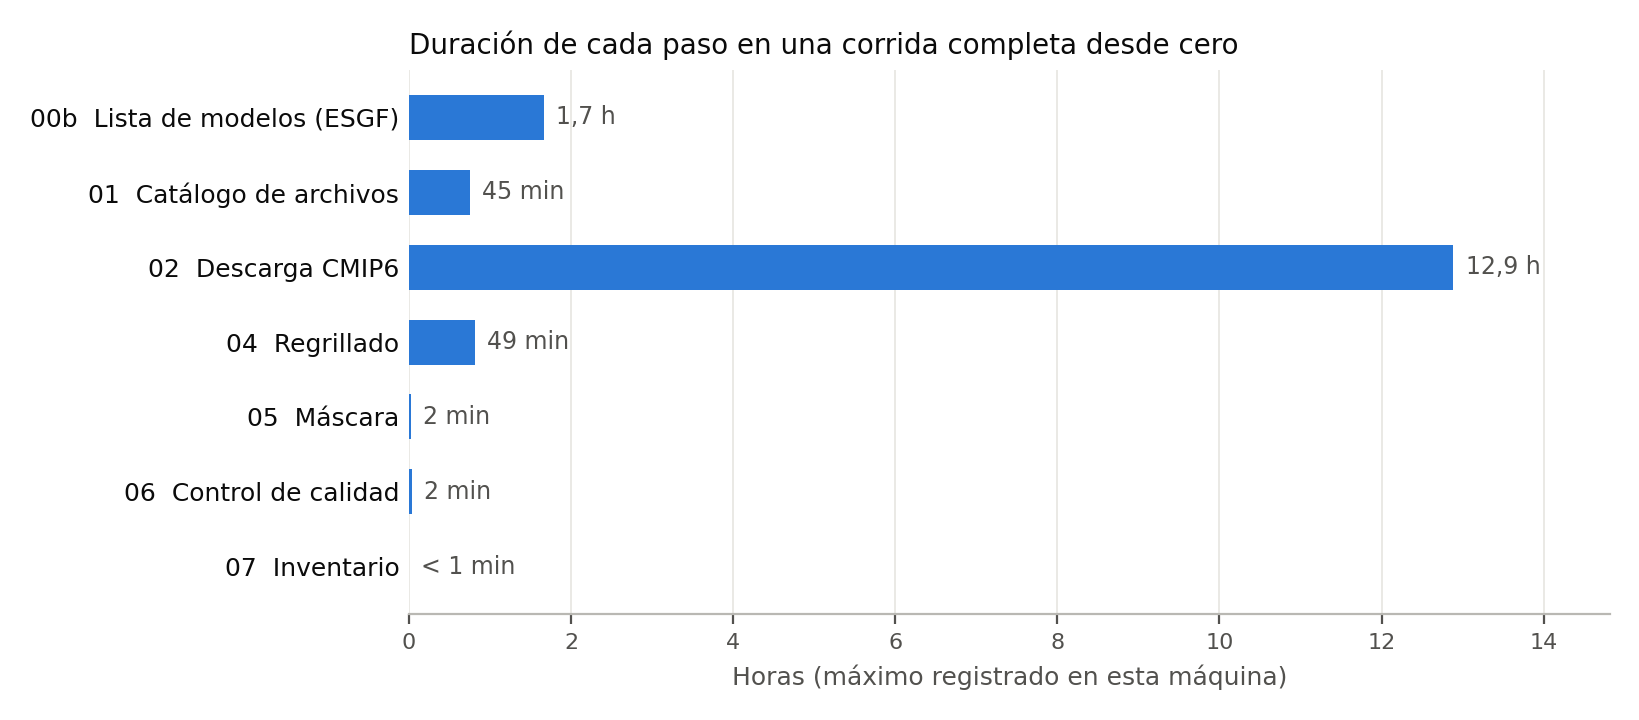
\includegraphics[width=0.92\textwidth]{figuras/anexo_tiempos.png}
\caption{Duración máxima registrada por paso (\texttt{logs/step\_timings.csv}). Los tiempos dependen de la conexión y del estado de los servidores de ESGF.}
\label{fig:tiempos}
\end{figure}

% ============================================================
\section{Dónde quedan los resultados}
% ============================================================

\noindent\begin{minipage}{\linewidth}
\begin{lstlisting}[basicstyle=\ttfamily\footnotesize]
smn_toe/
|-- data/
|   |-- raw/                      <- datos descargados, sin tocar (73 GB)
|   |-- interim/                  <- catálogo de descargas e intermedios
|   `-- processed/
|       |-- masked/               <- ARCHIVOS FINALES: tos_<modelo>_<experimento>.nc
|       |                            y ersstv5_region.nc (160 + 1 archivos)
|       |-- qc_report.csv         <- control de calidad, una fila por archivo
|       `-- models_inventory_final.csv  <- lista final: selected=True / False
|-- figures/                      <- figuras generadas automáticamente
|-- logs/
|   |-- pipeline.log              <- todo lo que se mostró en pantalla
|   `-- run_report_<fecha>.txt    <- resumen de estado de cada corrida
`-- informe/
    |-- model_registry.csv        <- código M001-M102, institución, país, resolución
    `-- entregable_update.tar.gz  <- paquete con todo lo necesario para el informe
\end{lstlisting}
\end{minipage}

\subsection{Cómo revisar los resultados}

\textbf{¿Cuántos modelos quedaron seleccionados?} (debe responder 40):
\begin{lstlisting}
grep -c ",True$" data/processed/models_inventory_final.csv
\end{lstlisting}

\textbf{¿Hubo algún archivo rechazado en el control de calidad?} (debe responder 0):
\begin{lstlisting}
grep -c ",FAIL," data/processed/qc_report.csv
\end{lstlisting}

\textbf{Ver una tabla CSV ordenada en columnas:}
\begin{lstlisting}
column -s, -t < data/processed/models_inventory_final.csv | less
\end{lstlisting}
(se sale de \texttt{less} con la tecla \texttt{q}).

\textbf{Ver qué contiene un archivo de datos:}
\begin{lstlisting}
conda activate smn_toe
cdo sinfo data/processed/masked/tos_ACCESS-CM2_historical.nc
\end{lstlisting}

El archivo \texttt{qc\_report.csv} tiene una fila por archivo: modelo, experimento, TSM mínima y máxima (°C), número de meses, si pasa el rango físico (\texttt{ok\_range}), si pasa la cobertura temporal (\texttt{ok\_length}) y el estado final (\texttt{PASS} o \texttt{FAIL}). El reporte \texttt{logs/run\_report\_<fecha>.txt} clasifica los modelos de la lista de descarga en: descargados completos, con descarga parcial, procesados, descargados pero sin procesar y pendientes en fuentes alternativas.

% ============================================================
\section{Qué hace cada paso (detalle técnico)}
\label{sec:pasos}
% ============================================================

Esta sección describe la lógica de cada script por su nombre y ruta, sin reproducir el código, que está disponible en el repositorio \archivo{smn_toe}. El flujograma de la Sección~6 del informe muestra el orden de los pasos; aquí se describe qué hace cada uno y qué controles incorpora.

\subsection{Paso 00 -- \texttt{scripts/00\_setup\_env.sh}}
Verifica las dependencias (\texttt{cdo}, \texttt{wget}, \texttt{python3} con el paquete \texttt{requests}) y crea la estructura de carpetas de datos y registros. No instala nada: si falta una herramienta, falla al inicio con un mensaje claro. La adquisición de datos se hace por HTTP directo contra ESGF y NOAA PSL, porque el repositorio público de CMIP6 en la nube de Amazon está en formato Zarr, incompatible con CDO, y no existe un equivalente para ERSSTv5.

\subsection{Paso 00b -- \texttt{scripts/00b\_build\_model\_list.py}}
Consulta el índice del nodo principal de ESGF (ORNL) y enumera todos los modelos CMIP6 que publican \texttt{tos}/\texttt{Omon}, que son 102. Para cada uno exige \texttt{historical} (o su equivalente \texttt{hist-1950} de HighResMIP), que busca también en nodos alternativos si el nodo principal no lo tiene indexado. Exige además los tres escenarios SSP configurados y retiene solo las variantes de grilla (\archivo{grid_label}) que cubren los cuatro experimentos; entre ellas elige la de mayor \archivo{nominal_resolution}, es decir, la más gruesa, convertida a kilómetros si el vocabulario la expresa en grados. Los modelos que califican quedan en \archivo{config/models_seed_cmip6.csv}. Para todos los modelos inspeccionados, el script escribe además \archivo{informe/model_availability_priority.csv}, con la disponibilidad 0/1 por experimento. Antes de repetir el barrido completo, que tarda más de una hora, hace una consulta rápida del número de modelos disponibles y solo rehace el barrido si ese número cambió.

\subsection{Paso 00c -- \texttt{scripts/00c\_check\_paper\_models.py} (diagnóstico manual)}
Busca los nombres de modelos CMIP6 citados en los resúmenes de la bibliografía del proyecto (una carpeta local de archivos Markdown, externa al repositorio) y los compara con la lista del Paso~00b. Los citados que no están en la lista se escriben en \archivo{config/models_missing_from_esgf.csv}, como candidatos para las fuentes alternativas. No forma parte de la secuencia automática de \texttt{run.sh}.

\subsection{Paso 01 -- \texttt{scripts/01\_query\_esgf\_catalog.py}}
Para cada modelo de la lista, consulta el nodo LLNL de ESGF y determina el miembro de ensamble (\archivo{variant_label}) común a los cuatro experimentos, prefiriendo \texttt{r1i1p1f1}. Escribe el catálogo \archivo{data/interim/models_catalog_status.csv} (estado por modelo, fuente, miembro y número acumulado de intentos de búsqueda) y las direcciones de descarga en \archivo{data/interim/esgf_file_urls.json}. Si el catálogo ya existe, no vuelve a consultar ESGF; para forzar una consulta nueva hay que borrar ambos archivos.

La búsqueda de archivos recorre el índice de ESGF por páginas hasta traer la lista completa. Un corte de red a mitad del recorrido puede truncar la lista sin mostrar error: en pruebas, la misma búsqueda de \texttt{EC-Earth3 historical} devolvió 107, 121 o 165 archivos según la corrida (165 es el total real). Por eso, si el recorrido se interrumpe, se repite completo desde el inicio, aquí y en el Paso~02b.

\subsection{Paso 02 -- descarga en cascada}
\archivo{scripts/02_download_all_sources.sh} encadena tres fuentes, cada una como respaldo automático de la anterior:
\begin{enumerate}[label=(\alph*)]
\item \archivo{02_download_cmip6_chunks.sh}: descarga HTTP directa con las direcciones del Paso~01. Cada dirección se reintenta tres veces, con una pausa breve, antes de pasar a la siguiente réplica. Es necesario para modelos que publican un archivo por año (hasta 165 archivos solo para \texttt{historical}), donde un corte transitorio en algún archivo es probable.
\item \archivo{02b_search_alt_esgf_nodes.py}: para los modelos que el nodo principal no resolvió, repite la búsqueda en ocho índices alternativos de la federación (CEDA, DKRZ, IPSL, NSC y NCI con la interfaz clásica, y ORNL, DKRZ y ESGF-West con la interfaz Metagrid), porque un modelo puede faltar en un índice por problemas de replicación y estar en otro.
\item \archivo{02c_download_copernicus_cds.py}: último recurso, solo para los modelos de \archivo{config/models_copernicus_available.csv}, la lista de modelos del conjunto \texttt{projections-cmip6} de Copernicus. Estar en la lista no garantiza que CDS tenga todos los experimentos; muchos pedidos de modelos poco replicados fallan con \texttt{RoocsValueError}. Requiere credenciales personales (\texttt{\textasciitilde/.cdsapirc}); sin ellas el paso se omite sin detener el resto.
\end{enumerate}
Antes de las fuentes (b) y (c), si hay modelos pendientes y la sesión es interactiva, el script pregunta si se desea intentarlas. Espera 15\,s y, sin respuesta, continúa como si fuera afirmativa, de modo que nunca bloquea una corrida desatendida. \texttt{run.sh} invoca este paso a través de \archivo{scripts/run_download_if_idle.sh}, que no lanza una segunda descarga si ya hay una en curso. Un modelo que agota (b) y (c) sin resolverse suma un intento en el catálogo; con tres intentos en corridas distintas deja de reintentarse hasta que se borre el catálogo.

\subsection{Paso 03 -- \texttt{scripts/03\_download\_ersstv5.sh}}
Descarga ERSSTv5 desde NOAA PSL una sola vez y la recorta con CDO a la ventana de descarga: toda la franja tropical, 0°--360° y 30°S--30°N (\texttt{config/domains.yaml}).

\subsection{Paso 04 -- \texttt{scripts/04\_process\_to\_common\_grid.sh}}
Para cada modelo y experimento:
\begin{enumerate}[label=(\arabic*)]
\item Usa solo los archivos crudos de la variante de grilla registrada en el catálogo. Es necesario porque una misma carpeta puede contener archivos de dos grillas del mismo periodo (ocurre con \texttt{CESM2}, con \texttt{gn} y \texttt{gr}), y al fusionarlos cada mes quedaría duplicado.
\item Descarta toda variable distinta de \texttt{tos} antes de regrillar, porque algunos modelos de malla curvilínea, como IPSL-CM6A-LR, incluyen variables auxiliares que hacen fallar a CDO.
\item Calcula una vez por modelo los pesos de interpolación hacia la grilla de ERSSTv5: conservativa (\texttt{gencon}) para mallas no estructuradas, como la de AWI-CM-1-1-MR, y bilineal (\texttt{genbil}) para el resto. Si los pesos del modelo fallan en un experimento, se recalculan pesos propios para ese experimento.
\item Fusiona en el tiempo los fragmentos ya regrillados y recorta al rango de años del experimento.
\item Asigna calendario \texttt{standard} si falta el atributo.
\item Convierte Kelvin a grados Celsius según el valor y no según el atributo: resta 273{,}15 solo si la media en Niño~3.4 es mayor o igual a 100. La regla es necesaria porque hay archivos que declaran \texttt{degC} pero contienen valores en Kelvin, como uno de GISS-E2-1-G (\texttt{ssp585}).
\item Verifica que el resultado tenga exactamente la misma lista de meses (año y mes, no solo el conteo) que los archivos crudos de la grilla correcta; si no coincide, descarta el resultado para reprocesarlo en la corrida siguiente.
\end{enumerate}
La comparación se hace contra lo que publican los archivos descargados y no contra un calendario ideal. Así, un modelo que publica permanentemente menos años de los pedidos se acepta tal cual: CAMS-CSM1-0 termina sus escenarios en 2099, e IITM-ESM empieza \texttt{historical} en 1900 y termina sus escenarios en 2098 o 2099.

\subsection{Paso 05 -- \texttt{scripts/05\_apply\_ocean\_mask.py}}
Construye una máscara océano-tierra derivada de ERSSTv5: un punto es océano si tiene al menos un valor válido en algún mes del registro. No usa la fracción de tierra propia de cada modelo (\texttt{sftlf}), de modo que la observación y todos los modelos comparten exactamente los mismos puntos válidos, condición necesaria para compararlos punto a punto. Se implementa en Python (\texttt{netCDF4}/\texttt{numpy}) porque la operación equivalente en CDO, aplicada sobre el valor de relleno, no propaga correctamente la máscara y marca como océano todo el dominio, incluida la tierra. Además aplica un filtro por valor físico: todo punto con $|\text{valor}| > 400$ pasa a \texttt{NaN}, independientemente de la máscara. El filtro es necesario porque FGOALS-f3-L contiene, en puntos que ERSSTv5 considera océano, un valor de relleno ($\sim$10$^{35}$) que el regrillado no reconoce como faltante; gracias a este filtro el modelo puede incorporarse al inventario.

\subsection{Paso 06 -- \texttt{scripts/06\_qc\_checks.py}}
Control de calidad automático de cada archivo procesado:
\begin{itemize}
\item \textbf{Rango físico}: la TSM debe estar entre $-2$ y 45\,°C. El límite superior considera que la franja tropical incluye mares marginales cálidos: en el mar Rojo y el golfo Pérsico algunos modelos alcanzan, de forma plausible, entre 39 y 41\,°C hacia 2100 en SSP3-7.0 y SSP5-8.5.
\item \textbf{Cobertura temporal}: en los escenarios SSP se admite hasta un 10\,\% menos de los meses esperados; en \texttt{historical} se exige que el registro llegue más allá de 1950, porque algunos modelos válidos no empiezan en 1850 (IITM-ESM empieza en 1900).
\end{itemize}
El resultado se escribe en \archivo{data/processed/qc_report.csv}. Las métricas se recalculan para todos los archivos en cada corrida, sin caché: un resultado guardado por nombre de archivo podría quedar desactualizado cuando un archivo se reprocesa. Como el control tarda menos de un minuto, recalcular siempre es la opción más segura. La exactitud de la cobertura la garantiza la verificación mes a mes del Paso~04; en la corrida final, los 40 \texttt{historical} terminan en 2014 y todos los archivos tienen sus meses completos.

\subsection{Paso 07 -- \texttt{scripts/07\_build\_inventory\_report.py}}
Combina el resultado del Paso~06 con la resolución de grilla (obtenida con \texttt{cdo griddes}) en \archivo{data/processed/models_inventory_final.csv}. Un modelo queda \texttt{selected=True} solo si aprueban el control de calidad los cuatro experimentos requeridos. Los cuatro se exigen explícitamente, en lugar de compararlos con los experimentos intentados, para que un modelo con descarga parcial no pueda quedar seleccionado aunque lo descargado apruebe.

\subsection{Reporte de estado -- \texttt{scripts/generate\_status\_report.py}}
Al final de cada corrida de \texttt{run.sh}, sin importar el rango de pasos, se escribe \archivo{logs/run_report_<fecha>.txt}, que clasifica cada modelo como descargado completo, con descarga parcial, procesado, descargado pero sin procesar, o pendiente de fuentes alternativas.


\clearpage
% ============================================================
\section{Problemas frecuentes}
% ============================================================

\begin{longtable}{@{}L{5.2cm}L{\dimexpr\textwidth-5.2cm-2\tabcolsep\relax}@{}}
\toprule
Mensaje o síntoma & Qué hacer \\
\midrule\endhead
\texttt{conda: command not found} & Miniconda no está instalado, o la terminal se abrió antes de instalarlo. Cierre y abra la terminal; si persiste, repita el Paso~1 de la instalación. \\
\texttt{FALTA cdo} u otra herramienta al inicio & El entorno no se creó. Ejecute \texttt{conda env create -f environment.yml}. \\
\texttt{Permission denied} al ejecutar \texttt{./run.sh} & Ejecute \texttt{chmod +x run.sh} una vez. \\
``Descarga ya en curso en otro proceso'' & Ya hay una descarga corriendo, por ejemplo en segundo plano. Es normal: espere a que termine y vuelva a ejecutar. \\
``se omite'' en Copernicus / falta \texttt{.cdsapirc} & No hay credenciales de Copernicus. Es opcional; el resto del \emph{pipeline} sigue. \\
La descarga se detuvo o se cortó la red & Vuelva a ejecutar el mismo comando; continúa donde quedó. \\
Un modelo ``agotó 3 intentos'' & No se volverá a buscar automáticamente. Para reintentar desde cero, borre \texttt{data/interim/models\_catalog\_status.csv} y \texttt{data/interim/esgf\_file\_urls.json} y ejecute de nuevo. \\
Disco lleno (\texttt{No space left on device}) & Libere espacio; con \texttt{du -sh data/*} se ve qué ocupa más. No borre \texttt{data/processed/}. \\
Las figuras no reflejan los últimos cambios & Ver el aviso de la Sección~\ref{sec:ejecutar}. \\
\bottomrule
\end{longtable}

% ============================================================
\section{Qué se espera hacer con estos datos}
% ============================================================

El Entregable~1 deja listo el dato. Los tres entregables siguientes lo usan en este orden (Figura~\ref{fig:ruta}): el Entregable~2 evalúa qué modelos representan mejor el ENOS, el Entregable~3 proyecta los cambios futuros y el Entregable~4 estima la incertidumbre y el tiempo de emergencia.

\begin{figure}[H]
\centering
\begin{tikzpicture}[font=\small,
  hito/.style={circle,draw=acento,fill=acento,minimum size=8pt,inner sep=0pt},
  hecho/.style={circle,draw=verde!80!black,fill=verde,minimum size=8pt,inner sep=0pt},
  caja/.style={draw=tinta2!60,fill=white,rounded corners=3pt,text width=3.25cm,align=left,inner sep=5pt,font=\scriptsize}]
\draw[very thick,tinta2!50] (0,0) -- (14.6,0);
\foreach \x/\d/\e/\s in {0.9/25/E1/hecho, 4.9/50/E2/hito, 8.9/80/E3/hito, 12.9/110/E4/hito}{
  \node[\s] at (\x,0) {};
  \node[font=\small\bfseries,above=5pt] at (\x,0) {\e};
  \node[font=\scriptsize,text=tinta2,below=5pt] at (\x,0) {día \d};
}
\node[caja,anchor=north] at (0.9,-0.8) {\textbf{Datos listos} (este entregable)\\[2pt]40 modelos $\times$ 4 experimentos; ERSSTv5; control de calidad; revisión de métodos de TOE.};
\node[caja,anchor=north] at (4.9,-0.8) {\textbf{Evaluar modelos}\\[2pt]climatología, ciclo anual, sesgos, diagrama de Taylor; ONI, RONI, ICEN; selección de los mejores modelos.};
\node[caja,anchor=north] at (8.9,-0.8) {\textbf{Proyectar}\\[2pt]cambios de la TSM media y de la variabilidad en 2036--2065 y 2071--2100; eventos extremos con ONI e ICEN.};
\node[caja,anchor=north] at (12.9,-0.8) {\textbf{Incertidumbre y TOE}\\[2pt]variabilidad interna, modelo y escenario; señal-ruido; TOE con M1 y ToD; estudio final.};
\end{tikzpicture}
\caption{Hoja de ruta del servicio. Los días se cuentan desde la notificación de la orden de servicio, según los términos de referencia.}
\label{fig:ruta}
\end{figure}

Para el Entregable~2 se usan directamente los archivos de \texttt{data/processed/masked/} y la lista de \texttt{models\_inventory\_final.csv}: no hace falta volver a descargar nada.

\clearpage
% ============================================================
\section{Estructura del repositorio}
% ============================================================

Para quien necesite ubicar un script concreto:

\begin{lstlisting}[basicstyle=\ttfamily\scriptsize]
smn_toe/
|-- run.sh                         # punto de entrada único
|-- environment.yml                # entorno conda (python, cdo, netcdf4, ...)
|-- README.md                      # documentación técnica detallada
|-- config/
|   |-- domains.yaml               # cajas Niño 3.4 / Niño 1+2 y ventana de descarga
|   |-- periods.yaml               # periodos y escenarios
|   |-- models_missing_from_esgf.csv       # candidatos de fuente alternativa (00c)
|   |-- models_no_encontrado_44.csv        # modelos sin algún experimento en ninguna fuente
|   |-- models_copernicus_available.csv    # modelos ofrecidos por Copernicus (02c)
|   |-- models_copernicus_ssp245_whitelist.csv  # referencia histórica, sin uso
|   `-- CMIP6_institution_id.json          # vocabulario oficial CMIP6: institución -> país
|-- scripts/
|   |-- 00_setup_env.sh            # verifica herramientas y crea carpetas
|   |-- 00b_build_model_list.py    # universo de modelos (ESGF, nodo ORNL)
|   |-- 00c_check_paper_models.py  # diagnóstico manual, no lo ejecuta run.sh
|   |-- 01_query_esgf_catalog.py   # catálogo de archivos (ESGF, nodo LLNL)
|   |-- 02_download_all_sources.sh # descarga en cascada 02a -> 02b -> 02c
|   |-- 02_download_cmip6_chunks.sh, 02b_search_alt_esgf_nodes.py,
|   |   02c_download_copernicus_cds.py, run_download_if_idle.sh
|   |-- 03_download_ersstv5.sh
|   |-- 04_process_to_common_grid.sh
|   |-- 05_apply_ocean_mask.py
|   |-- 06_qc_checks.py
|   |-- 07_build_inventory_report.py
|   |-- build_model_registry.py    # códigos M001-M102
|   |-- generate_status_report.py  # logs/run_report_<fecha>.txt
|   |-- preflight_report.py        # reporte previo con estimación de tiempo
|   |-- pipeline_config.py, pipeline_timing.py   # configuración y tiempos
|   |-- bundle_deliverable_update.py             # paquete .tar.gz
|   `-- plot_*.py                  # las cinco figuras automáticas
`-- data/, figures/, logs/, informe/   # salidas (Sección 6)
\end{lstlisting}

\end{document}
